\documentclass[twoside]{article}
\usepackage[a4paper]{geometry}
\geometry{verbose,tmargin=2.5cm,bmargin=2cm,lmargin=2cm,rmargin=2cm}
\usepackage{fancyhdr}
\pagestyle{fancy}

% nastavení pisma a~češtiny
\usepackage{lmodern}
\usepackage[T1]{fontenc}
\usepackage[utf8]{inputenc}
\usepackage[czech]{babel}

% odkazy
\usepackage{url}

\usepackage{float}
% vícesloupcové tabulky
\usepackage{multirow}
\usepackage{listings}
\usepackage{xcolor}
\usepackage{amssymb}
\usepackage{gensymb}
\usepackage{bbold}
\usepackage{amsmath}
\usepackage{siunitx}
\usepackage{mathtools}
\usepackage{commath}
\usepackage{xcolor}

% vnořené popisky obrázků
\usepackage{subcaption}

% automatická konverze EPS 
\usepackage{graphicx} 
\usepackage{epstopdf}
\epstopdfsetup{update}

\graphicspath{{./images}}

% odkazy a~záložky
\usepackage[unicode=true, bookmarks=true,bookmarksnumbered=true,
bookmarksopen=false, breaklinks=false,pdfborder={0 0 0},
pdfpagemode=UseNone,backref=false,colorlinks=true] {hyperref}


% Poznámky při překladu
\usepackage{xkeyval}	% Inline todonotes
\usepackage[textsize = footnotesize]{todonotes}
\presetkeys{todonotes}{inline}{}

%https://tex.stackexchange.com/questions/2783/bold-calligraphic-typeface
\DeclareMathAlphabet\mathbfcal{OMS}{cmsy}{b}{n}

% enumerate zacina s pismenem
\renewcommand{\theenumi}{\alph{enumi}}

% smaz aktualni page layout
\fancyhf{}
% zahlavi
\usepackage{titling}
\fancyhf[HC]{\thetitle}
\fancyhf[HLE,HRO]{\theauthor}
\fancyhf[HRE,HLO]{\today}
 %zapati
\fancyhf[FLE,FRO]{\thepage}

% údaje o autorovi
\title{VSY - Integrační voltmetr - dokumentace}
\author{Vojtěch Michal}
\date{\today}

%customize code listing
\definecolor{codegreen}{rgb}{0,0.6,0}
\definecolor{codegray}{rgb}{0.5,0.5,0.5}
\definecolor{codepurple}{rgb}{0.58,0,0.82}
\definecolor{backcolour}{rgb}{0.95,0.95,0.92}

\lstdefinestyle{mystyle}{
    backgroundcolor=\color{backcolour},   
    commentstyle=\color{codegreen},
    keywordstyle=\color{magenta},
    numberstyle=\tiny\color{codegray},
    stringstyle=\color{codepurple},
    basicstyle=\ttfamily\footnotesize,
    breakatwhitespace=false,         
    breaklines=true,                 
    captionpos=b,                    
    keepspaces=true,                 
    numbers=left,                    
    numbersep=5pt,                  
    showspaces=false,                
    showstringspaces=false,
    showtabs=false,                  
    tabsize=2
}

\lstset{style=mystyle}

\begin{document}

\maketitle

\section{Stanovení hodnot součástek}

\subsection{Parametry integrátoru}

Pro invertující integrátor s operačním zesilovačem a prvky $R$, $C$ platí závislost výstupního napětí 
$u_o(t)$ na vstupním $u_i(t)$ daná vztahem
\begin{equation}
    u_o(t) = - \frac{1}{C} \int_0^t \frac{u_i(\tau)}{R} \text{d}\tau = \frac{-1}{R\cdot C} \int_0^t u_i(t) \text{d}t.
\end{equation}
Protože je integrátor po zakončení každé integrační periody vrácen do nuly (kondenzátor $C$ je vybit), lze
bez újmy na obecnosti předpokládat nulové počáteční podmínky. Operační zesilovače mají symetrické napájení $\pm$ 5 V 
a je silně nežádoucí, aby se jejich výstup dostal blízko oblasti saturace. Proto je potřeba volit parametry $R$, $C$ tak,
aby zvolená doba integrace při připojení maximálního vstupního napětí nedosáhla saturace integrátoru.

Pro zvolenou integrační dobu $T_1 = 40~\text{ms}$ volím maximální žádoucí napětí $U_{o_\text{max}} = 3,3$ V, neboť poté bude možné 
pro případné ladění obvodu použít ADC na dalším nucleu. Dále volíme $C = 220$ nF. Pro vstupní rozsah $u_i \in \langle -2, 0 \rangle$ V platí
\begin{equation}
    3,3~\text{V} \ge U_{o_\text{max}} = - \frac{1}{R \cdot C} \int_0^{T_1} u_{i_\text{min}}(\tau) \text{d} \tau = \frac{1}{R \cdot C} \cdot T_1 \cdot \abs{u_{i_\text{min}}},
\end{equation}
což je rovnice pro jednu neznámou $R$. Po úpravě
\begin{equation}
    R \ge \frac{T_1 \cdot \abs{u_{i_\text{min}}}}{U_{o_\text{max}} \cdot C}.
\end{equation}
Pro výše uvedené parametry je to například
\begin{equation}
    R \ge \frac{0,04~\text{s} \cdot 2~\text{V}}{3,3~\text{V} \cdot 220 \cdot 10^{-9}~\text{F}} \approx 110~\text{k}\Omega.
\end{equation}
S použitím $R = 200~\text{k}\Omega$ budeme mít dvojnásobnou jistotu, že bude bezpečné na výstup integrátoru připojit ADC.

\subsection{Parametry regulátoru}

K napěťové referenci TL431 je potřeba doplnit kondenzátor (doporučeno $C_\text{b} = 22~\mu \text{F}$) a rezistor $R_\text{R}$, kterým
potečou cca 2 mA při napěťovém úbytku 2,5 V. Použitelná hodnota je tedy $R_\text{R}$ = 470 R.

\section{Struktura aplikace}

Mikrokontroler třemi logickými signály \textbf{S2}, \textbf{S1}, \textbf{S0} (souhrně \textbf{MUX\_SEL}) nastavuje
multiplexor na vstupu analogového front-endu. Mapování hodnot \textbf{MUX\_SEL} na zvolené kanály
a jejich význam jsou v tabulce \ref{table:mux}. Pro detailnější porozumění významu jednotlivých kanálů
konzultujte schéma zapojení. Očekávané mapování signálů na piny Nucleo desky je uvedeno v tabulce \ref{table:pinout}.

Vstupní signál \textbf{MCU\_IN} je přes ochranný rezistor připojen na výstup komparátoru.
Detekováním hran na signálu \textbf{MCU\_IN} lze identifikovat průchody napětí na integrátoru $U_{\text{int}}$ nulou.
Na mikrokontroleru je signál připojen na timer, jenž zajišťuje přesné odměřování času mezi hranami.
Pro více informací viz \ref{sec:detail}

\begin{table}[htbp]
    \centering
    \begin{tabular}{c|c|c|c|c}
        \textbf{S2} & \textbf{S1} & \textbf{S0} & \textbf{jméno kanálu} & \textbf{význam}\\ \hline
        0 & 0 & 0 & $U_{\text{in}}$ & neznámé vstupní napětí \\
        0 & 0 & 1 & GND & hladina nulového potenciálu \\
        0 & 1 & x & $U_{\text{ref}}$ & referenční napětí cca 2,51 V, generované obvodem TL431\\
        1 & x & x & $U_{\text{FB}}$ & feedback z výstupu komparátoru
    \end{tabular}
    \caption{Mapování hodnot \textbf{MUX\_SEL} na vstupní kanály multiplexoru}
    \label{table:mux}
\end{table}

\begin{table}[htbp]
    \centering
    \begin{tabular}{c|c|c|c}
        \textbf{signál} & \textbf{periferie} & \textbf{pin STM32} & \textbf{pin Arduino konektoru} \\ \hline 
        \textbf{MCU\_IN} & TIM2\_CH1, timer trigger & PA0 & A0 \\
        \textbf{MCU\_IN} & TIM2\_CH3, input compare & PA9 & D8 \\
        \textbf{S1} & TIM2\_CH2, output compare & PA1 & A1 \\
        \textbf{S2} & GPIO & PC1 & A4 \\
        \textbf{S0} & GPIO & PC0 & A5 \\
        \textbf{USART2\_TX} & USART2 & PA2 & \textit{N/A} (přes ST-Link do PC)\\
        \textbf{USART2\_RX} & USART2 & PA3 & \textit{N/A} (přes ST-Link do PC)
    \end{tabular}
    \caption{Pinout mikrokontroleru}
    \label{table:pinout}
\end{table}


\section{Komunikační rozhraní}

Zařízení komunikuje po technologii UART, nastavení 115200 baud, 8 datových bitů, jeden stop bit,
bez parity. V rámci ST-Linku je přítomen UART<->USB převodník, který zajišťuje překlad komunikace pro PC.
Všechny příkazy přijímané zařízením nerozlišují velká a malá písmena a jsou dlouhé jeden znak
s výjimkou výzvy ke konfiguraci, která je detailně dokumentována v sekci \ref{sec:config}
V tabulce \ref{tab:commands} jsou uvedeny všechny příkazy použitelné pro řízení aplikace,
v její spodní polovině jsou konkrétní příkazy použitelné pro ladění kompenzaci chyby měření.

Pro navázání spojení s aplikací je doporučeno připojení pomocí standardního linuxového terminálu.
\begin{enumerate}
    \item Zjistěte číslo COM portu přiřazeného voltmetru (na Windows pomocí správce zařízení). Nechť je zařízení připojeno např na \textit{COM12}.
    \item Nastavte COM port na parametry komunikace \textit{stty -F /dev/ttyS12 115200 raw -parenb}
    \item Spusťte čtení z COM portu \text{cat /dev/ttyS12}.
    \item Spusťte zápis do COM portu \text{stty raw; cat > /dev/ttyS12} ve vedlejší instanci terminálu.
    \item Resetujte zařízení stiskem tlačítka. Ze zařízení by se měl objevit výpis \textit{"VoMi's dual slope integration ADC initialized and ready."}
\end{enumerate}

\begin{table}[htbp]
    \centering
    \begin{tabular}{c|c|c}
        \textbf{příkaz} & \textbf{funkce}  & \textbf{popis} \\ \hline
        \textbf{Q} & Reset & Resetuje mikrokontroler. Ekvivalentní stisku resetovacího tlačítka. \\
        \textbf{S} & Single & Spustí či zastaví \textbf{one-shot} měření s aktuálním nastavením \\
        \textbf{R} & Run & Spustí \textbf{kontinuální} měření s aktuálním nastavením \\
        \textbf{E} & Exit & Ukončí probíhající kontinuální měření\\
        \textbf{H} & Help & Vypíše seznam rozpoznávaných příkazů \\
        \textbf{C} & Configure & Vstoupí do konfiguračního módu (viz \ref{sec:config}) \\
        \textbf{I} & Info & Vypíše aktuální hodnoty konfiguračních parametrů (viz \ref{sec:config}) \\
        \hline
        \textbf{D} & Derivative & Přepne zařízení do režimu ladění sklonu charakteristiky \\       
        \textbf{O} & Offset & Přepne zařízení do režimu ladění konstantního posunutí charakteristiky \\       
        \textbf{+} & Inc Param &   Zvýší hodnotu parameteru zvoleného příkazy \textbf{D} či \textbf{O}\\       
        \textbf{-} & Dec Param &   Sníží hodnotu parameteru zvoleného příkazy \textbf{D} či \textbf{O}\\       
        \textbf{*} & Reset Param & Obnoví základní hodnotu parameteru zvoleného příkazy \textbf{D} či \textbf{O}\\       
    \end{tabular}
    \caption{Přehled příkazů rozeznávaných aplikací}
    \label{tab:commands}
\end{table}

\section{Konfigurace}
\label{sec:config}

Aplikace podporuje konfiguraci mnoha proměnných v reálném čase, všechny jsou uvedené v tabulce \ref{tab:config}.
Všechny parametry jsou škálované celočíselné hodnoty, nebo pravdivostní. U pravdivostních hodnot je nula interpretována
jako \textit{false} a jakékoli nenulové číslo interpretováno jako \textit{true}.

Konfiguraci je standardně možno měnit výhradně při deaktivovaném měření (zařízení v režimu \textit{idle}).
Výjimkou je ladění error correction koeficientů \textit{MEAS\_OFFSET} a \textit{MEAS\_SCALE}, které je možné
provádět průběžně i během měření. Stiskem kláves \textbf{D}erivative či \textbf{O}oofset lze přepínat mezi laděním sklonu a offsetu charakteristiky.
Po vybrání parametru k ladění je možné použitím kláves \textbf{+} a \textbf{-} měnit plynule hodnotu.
Aktuální hodnotu error correction parametrů lze získat spolu se všemi ostatními parametry pomocí příkazu \textbf{I}nfo.
Obnovení továrního nastavení parametru lze provést stiskem klávesy \textbf{*}.


\begin{table}[htbp]
    \centering
    \begin{tabular}{c|c|c|c}
        \textbf{jméno parametru} & \textbf{význam} & \textbf{reset value} & \textbf{jednotka} \\ \hline
        AVG\_LEN & Počet vzorků použitých k průměrování & 16 & -- \\
        OVERWRITE & Aktivuje přepisování předchozích měření novými vzorky & 1 & bool \\
        MEAS\_SCALE & Korekční faktor sklonu charakteristiky & 9967 & $10^{-4}$ \\
        MEAS\_OFFSET & Korekční faktor konstantního posunutí charakteristiky & -155 & 0.1 mV \\
        V\_REF & Hodnota napěťové reference zařízení & 2517 & mV \\
        SOFT\_START\_LEN & Délka fáze soft-start integračního cyklu & 800 & $\mu$s \\
        T1\_DUR & Délka fixní fáze integračního cyklu & 40 & ms \\
        PRINT\_SAMPLES & Nastavuje formát vypisovaných dat & 0 & bool
    \end{tabular}
    \caption{Přehled konfigurovatelných parametrů}
    \label{tab:config}
\end{table}


\section{Nastavení periferií}

Všechny vnitřní sběrnice v mikrokontroleru (AHB, APBx) běží na frekvenci 8 MHz.

Pro časování fáze \textit{soft start} je použita periferie TIM7, konfigurována na one pulse mode; update request source
je pouze přetečení vnitřního counteru, aby nebyla vyvolávána planá přerušení. Použitý prescaler je 8 (čítání s mikrosekundovým rozlišením).
V auto-reload registru ARR je vždy uložena hodnota délky fáze \textit{soft start} v mikrosekundách (v základu 800). V periferii i NVIC je povoleno přerušení.

Pro časování integrace je použita periferie TIM2. Jako interní trigger je zvolen neinvertovaný filtrovaný vstup z kanálu 1 (TI1FP1),
timer je provozován v \textit{gated mode}, kdy inkrementování registru CNT je podmíněno vysokou úrovní na interním triggeru (kanál 1 je připojen na signál \textbf{MCU\_IN}).
V periferii i jádře je povolen požadavek na přerušení od třetí capture/compare jednotky. Capture/compare unit 3 má jako vstup TIM2\_CH3, bez použití prescaleru nebo filtrování,
vstup je invertován (jednotka citlivá na sestupnou hranu). Capture/compare jednotka 2 je v režimu output compare. V základu vynucuje nízkou úroveň, v době měřicího cyklu je přepnuta na mód PWM2,
kdy je výstup v logické nule pro CNT <= CCR2. V CCR2 je zapsána délka doby t1 v mikrosekundách (v základu 40 000).

Komunikace s řídicím počítačem je realizována periferií USART2, baudrate prescaler $69~\frac{7}{16} = 69.4375$. Skutečný baudrate proto je $\frac{8\cdot 10^6}{69.4375} = 115211.52$ bps,
relativní chyba 0.01 \%. Je povolen vysílač i přijímač, aktivováno přerušení při příjmu znaku. Nastavení 8 datových bitů, 1 stop bit a bez parity je pro použitou periferii základní
a není tak potřeba měnit reset value registrů.

Pro určování času běhu aplikace je použita periferie SysTick, jako zdroj hodin je sběrncie AHB bez předděliček; je povoleno přerušení, perioda nastavena na 1 ms.


\section{Detailní popis chování aplikace}
\label{sec:detail}
Pro snazší vysvětlení chování zařízení jsou připojeny obrázky z osciloskopu připojeného na obvod během testování.
Na všech následujících obrázkách je použité stejné mapování kanálů osciloskopu uvedené v tabulce \ref{table:oscilloscope}.
Mezi obrázky se však liší časová základna i měřítko na vertikální ose. Velikost časové základny je na každém obrázku vidět
na horním okraji uprostřed. Měřítko na svislé ose je zobrazeno v levém dolním rohu obrázků.
Časové průběhy signálů během dvou po sobě jdoucích měřicích cyklů jsou vykresleny na obrázku \ref{fig:overview},
do kterého byly doplněny i názvy jednotlivých fází měřicího cyklu. Dílčí fáze převodu jsou popsány dále.

\begin{table}
    \centering
    \begin{tabular}{c|c|c}
        \textbf{kanál} & \textbf{barva} & \textbf{signál} \\ \hline
        1 & \textcolor{yellow}{\textbf{žlutá}} & napětí na integrátoru $U_{\text{int}}$ \\
        2 & \textcolor{green}{\textbf{zelená}} & výstup komparátoru \\
        3 & \textcolor{orange}{\textbf{oranžová}} & výstup multiplexoru (aktuálně integrované napětí)
    \end{tabular}
    \caption{Mapování kanálů osciloskopu na signály obvodu pro obrázky \ref{fig:overview} a další}
    \label{table:oscilloscope}
\end{table}

V režimu \textit{idle} je aktivován feedback z komparátoru zpět na vstup integrátoru a výstup integrátoru $U_{\text{int}}$ osciluje poblíž nuly s malou amplitudou (pod 1 mV).
Oscilují rovněž výstup komparátoru a ve fázi s ním výstup sledovače. Toto chování je vidět na levé straně obrázku \ref{fig:soft_start}.
Režim \textit{idle} je zvolen při inicializaci zařízení, mezi měřicími cykly a po skončení měření.

Na základě příkazu ze seriové linky odstartuje převodník proces měření napětí:
\begin{itemize}
    \item Ze stavu \textit{idle} přejde software do stavu \textit{soft start}.
    \item Vynucením aktivní (vysoké) úrovně na TIM2\_CH2 připojené na \textbf{S1} se připraví mux na připojení referenčního napětí $U_{\text{ref}}$.
    \item Uvedením \textbf{S2} do logické nuly se deaktivuje feedback. Tím se připojí na výstup muxu referenční napětí $U_{\text{ref}}$.
    \item Spustí se TIM7 odpočítávající dobu specifikovanou parametrem \textbf{soft\_start\_delay} (v základu 800 $\mu\text{s}$).
\end{itemize}

Po uplynutí specifikované doby vyvolá TIM7 přerušení. Protože bylo integrováno kladné napětí, výstup integrátoru je nyní pod nulou a tedy ořezaný signál z komparátoru
\textbf{MCU\_IN} je v logické nule. V obsluze přerušení:
\begin{itemize}
    \item Software přejde ze stavu \textit{soft start} do stavu \textit{measuring}.
    Ten není dále dělen, protože toto je poslední zásah ze strany jádra; dále bude zbytek měřicího procesu řídit kompletně hardware periferie TIM2.
    \item Software vygeneruje update TIM2 (vynulování registru CNT, případně aktualizace preloaded CCRx registrů).
    \item Aktivují se capture/compare jednotky peripferie TIM2.
    \item TIM2\_CH2 se přepne z vynucené aktivní úrovně na PWM2 mód (TIM2\_CH2 = 0 pro TIM2\_CNT <= TIM2\_CCR2).
    Tím je signál \textbf{S1} v nule a multiplexer se přepne z referenčního napětí na neznámé napětí $U_{\text{in}}$.
\end{itemize}
Přepnutím na neznámé záporné napětí začíná výstupní napětí integrátoru růst. V okamžiku průchodu $U_{\text{int}}$ hladinou nulového potenciálu přeběhne signál \textbf{MCU\_IN}
do logické jedničky, což spustí čítač uvnitř TIM2. Timer čeká na uběhnutí předem nastavené doby $T_1 = 40$ ms v TIM2\_CCR2. Po jejich uplynutí nastane compare event,
výstup TIM2\_CH2 (\textbf{S1}) jde do logické jedničky, čímž se místo neznámého napětí připojí na výstup multiplexoru kladné referenční napětí $U_{\text{ref}}$.
Začíná se odměřovat doba $T_2$ proměnlivé délky.
Integrováním kladného napětí začně poklesat napětí $U_{\text{int}}$, až opět dosáhne hladiny nulového potenciálu. Tehdy nastane sestupná hrana na signálu \textbf{MCU\_IN}, která
je detekována input capture jednotkou TIM2\_CH3. Nastává capture event, aktuální hodnota TIM2\_CNT je uložena to TIM2\_CCR3 a jádro dostane požadavek na přerušení.
Protože \textbf{MCU\_IN} je po sestupné hraně v logické nule, TIM2 se v týž okamžik sám deaktivuje.

V obsluze přerušení od TIM2 jsou vyčteny hodnoty registrů TIM2\_CCR3 a TIM2\_CCR2. Díky nastavení slave mode controlleru tak, aby timer čítal jen a tehdy, když je logický signál \textbf{MCU\_IN}
v logické jedničce, tedy výstup komparátoru je na kladném napájení, tedy $U_{\text{int}} > 0$ V, obsahuje registr TIM2\_CCR3 přesně dobu mezi vzestupným a sestupným průchodem napětí $U_{\text{int}}$ nulou,
tedy platí
\begin{equation}
    \text{TIM2\_CCR3} = T1 + T2.
\end{equation}

Neboť hodnota TIM2\_CCR2 byla přesně použita pro vygenerování doby $T1$, jejich odečtením je získána délka doby $T2$ v cyklech systémových hodin (8 cyklů na mikrosekundu, 125 ns na cyklus).
Následně je nastavením signálu \textbf{S2} aktivován na multiplexoru feedback. Systém přechází do stavu \textit{idle}.


\begin{figure}[htbp]
    \centering
    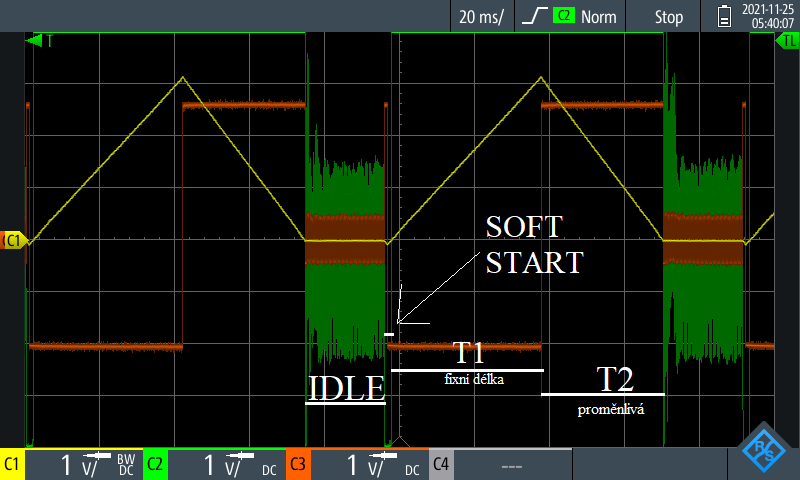
\includegraphics[width=\linewidth]{overview.png}
    \caption{Časové průběhy signálů během měření $U_{\text{in}}~\approx~U_{\text{FB}}$}
    \label{fig:overview}
\end{figure}

\begin{figure}[htbp]
    \centering
    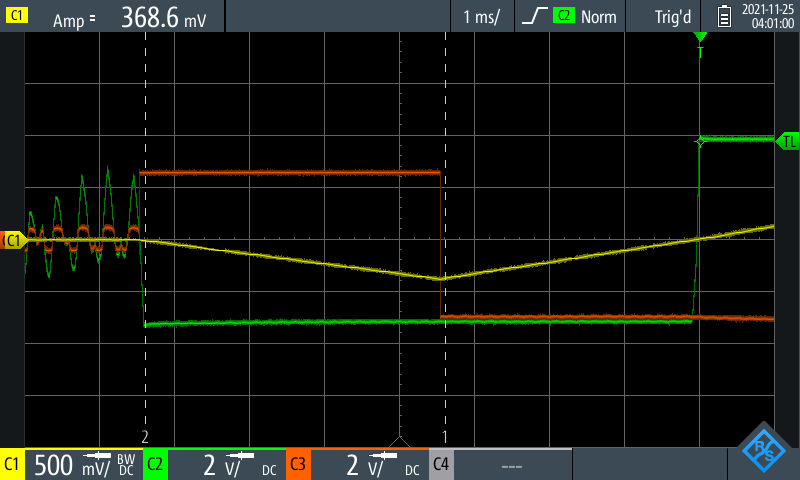
\includegraphics[width=\linewidth]{soft_start.png}
    \caption{Detail časového průběhu signálů během fáze \textit{soft start}}
    \label{fig:soft_start}
\end{figure}

\begin{figure}[htbp]
    \centering
    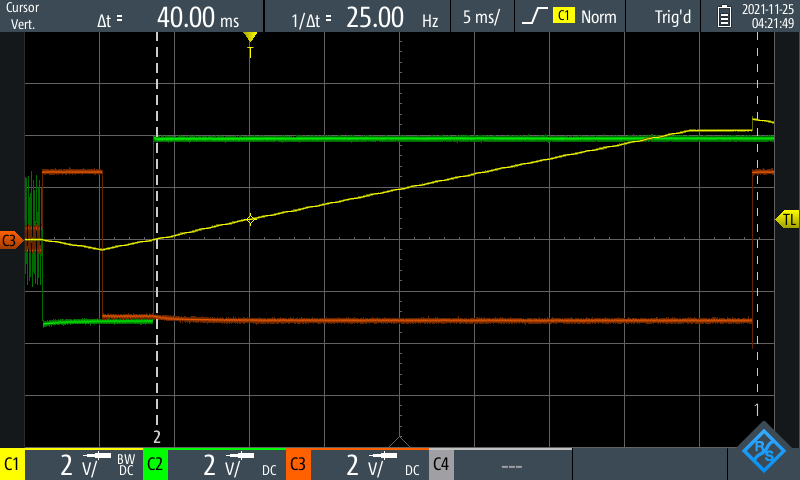
\includegraphics[width=\linewidth]{t1.png}
    \caption{Detail časového průběhu signálů během fáze $T_1$}
    \label{fig:t1}
\end{figure}

\begin{figure}[htbp]
    \centering
    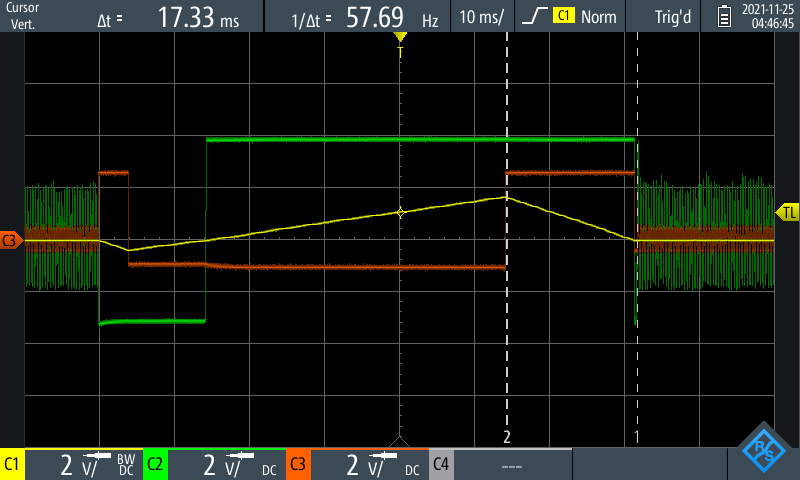
\includegraphics[width=\linewidth]{t2.png}
    \caption{Detail časového průběhu signálů během fáze $T_2$}
    \label{fig:t2}
\end{figure}

Na obrázku \ref{fig:uin_uref} je příklad časových průběhů měřicích cyklů v případě, kdy je měřené napětí blízké referenčnímu napětí $U_{\text{ref}}$.
Pomocí vertikálních kurzorů i časové základny je ukázáno, že doba odintegrovávání $T_2$ je přibližně rovno době $T_1$ = 40 ms.

\begin{figure}[htbp]
    \centering
    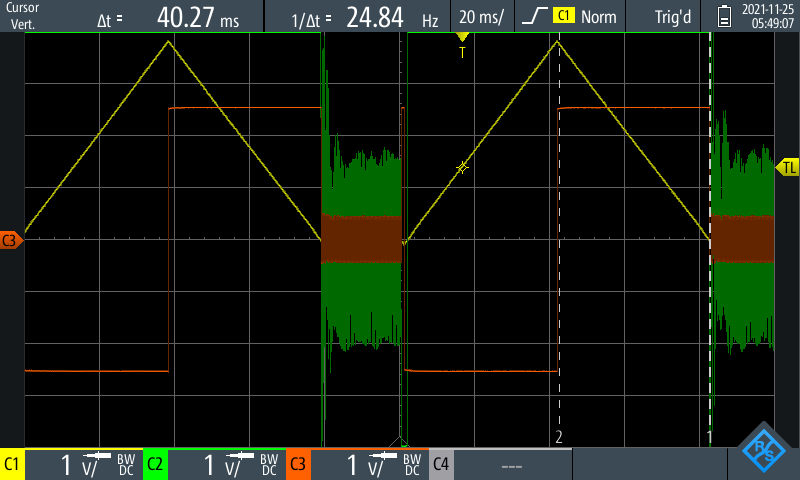
\includegraphics[width=\linewidth]{Uin_cca_Uref.png}
    \caption{Měřicí cyklus pro $U_{\text{ref}} \approx U_{\text{in}}$}
    \label{fig:uin_uref}
\end{figure}


\end{document} 